\chapter{Tools demonstration}
\label{cap:casestudy}

To ilustrate the whole process of generating test cases and extracting formal properties and how our implemented tools work, we will use as a case study the statechart model given in \ref{fig:stockUpdateEmail} and presented below as well for better consulting:

\begin{figure}[h]
\centering
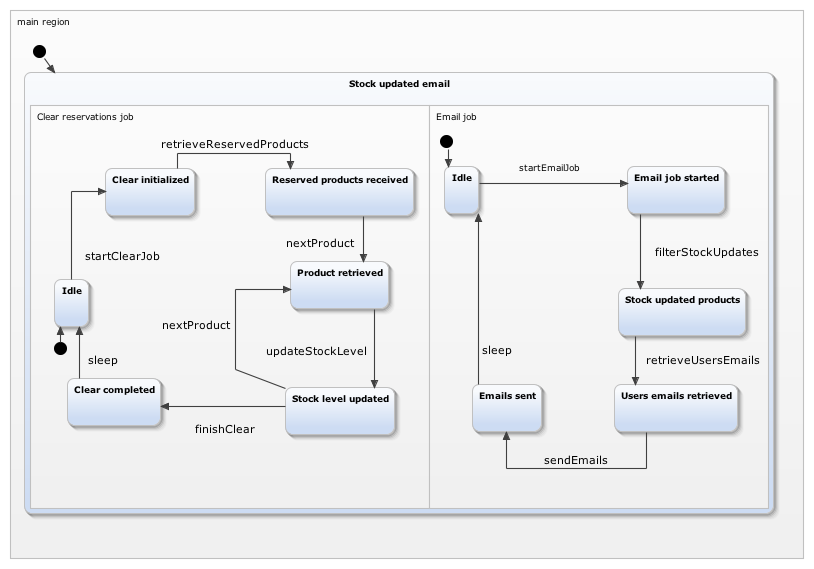
\includegraphics[width=15cm]{figuras/stockUpdateEmail}
\caption{\label{fig:stockUpdateEmail_2} Statechart model for concurrent jobs: clear reservations job and send email job}
\end{figure}

\section{Test case generation tool}

We start by running our test case generation tool and provide the path to the previous Yakindu statechart in our machine. We also select the $SPMF$ to already get the sequences in the $SPMF$ input format as displayed in figure \ref{fig:testGenTool_1}.

\begin{figure}[htb]
\centering
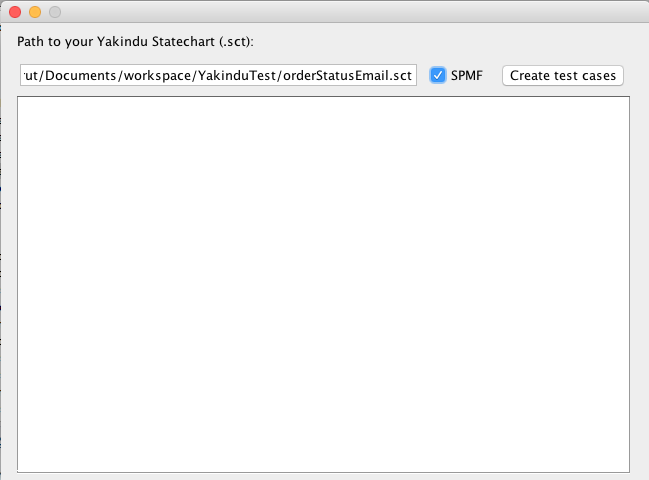
\includegraphics[width=10cm]{figuras/testGenTool_1}
\caption{\label{fig:testGenTool_1} Test generation tool.}
\end{figure}

By clicking on button \textit{Create test cases}, all test cases for the inputed statechart will be printed (figure \ref{fig:testGenTool_2}). The test paths will also be outputed in the $SPMF$ format as we can check in figure \ref{fig:testGenTool_3}.

\begin{figure}[htb]
\centering
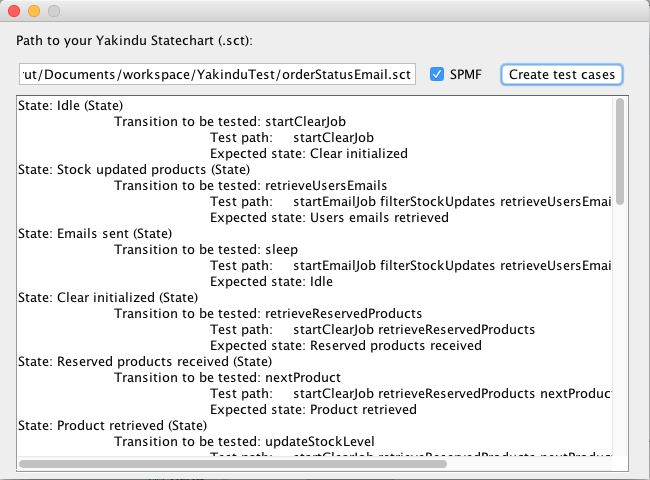
\includegraphics[width=10cm]{figuras/testGenTool_2}
\caption{\label{fig:testGenTool_2} Test cases created based on statechart \ref{fig:stockUpdateEmail_2}.}
\end{figure}

\begin{figure}[htb]
\centering
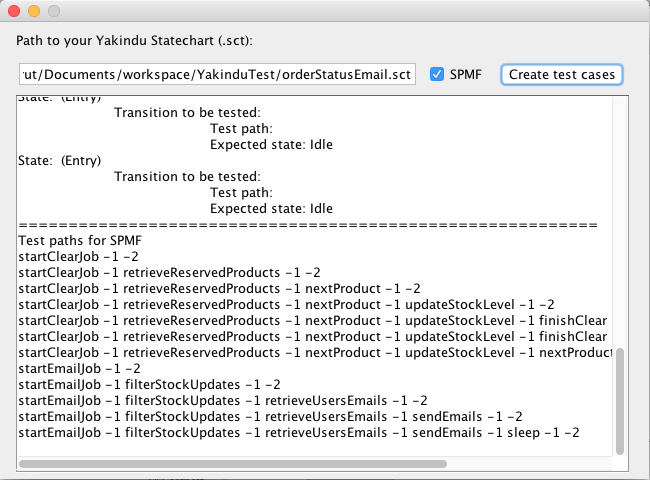
\includegraphics[width=10cm]{figuras/testGenTool_3}
\caption{\label{fig:testGenTool_3} Test paths in the $SPMF$ input format.}
\end{figure}

\section{Formal property specification tool}

Now, we save the $SPMF$ sequences in a separte file and start our tool to extract formal property specifications. We provide the path to the file where the previous $SPMF$ sequences were saved and a minimum support of $50\%$ (0.5), as shown in figure \ref{fig:propGenTool_1}.

\begin{figure}[htb]
\centering
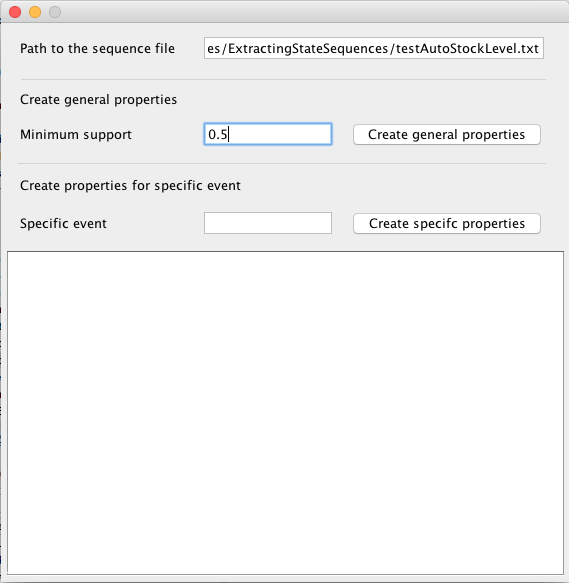
\includegraphics[width=10cm]{figuras/propGenTool_1}
\caption{\label{fig:propGenTool_1} Property generation tool.}
\end{figure}

By clicking on \textit{Create general properties}, response and existence properties will be defined based on the mining results. In figure \ref{propGenTool_2}, we can notice that one property was defined and that sequences 8, 9, 10, 11 and 12 were not used due to the mining phase. Note that the ID of each sequence is the correponding number of the line the sequence is written.

\begin{figure}[htb]
\centering
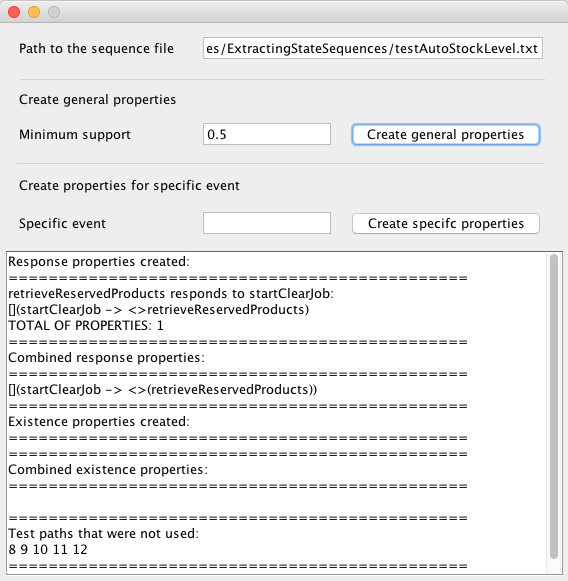
\includegraphics[width=10cm]{figuras/propGenTool_2}
\caption{\label{fig:propGenTool_2} Properties defined based on mining of the test cases from \ref{fig:stockUpdateEmail_2} with minimum support of $50\%$.}
\end{figure}

One import event from such left aside sequences is \textit{sendEmails}. We can then pass this event as input in the second text field to generate specific property specifications, which are displayed in figure \ref{fig:propGenTool_3}.

\begin{figure}[htb]
\centering
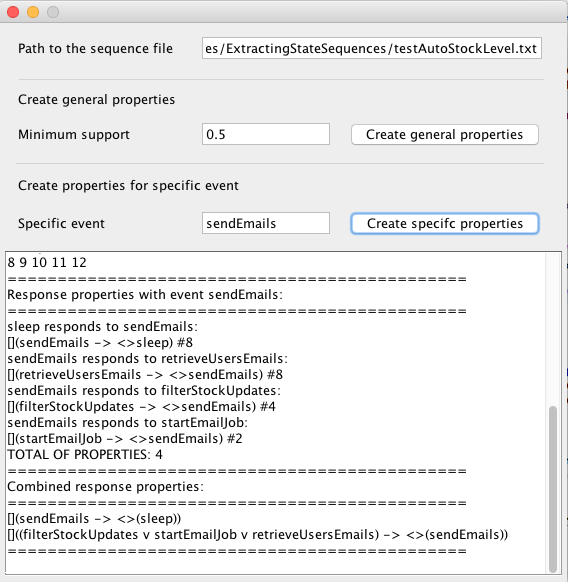
\includegraphics[width=10cm]{figuras/propGenTool_3}
\caption{\label{fig:propGenTool_3} Specific Properties defined for event \textit{sendEmails}.}
\end{figure}
